\section{スピンフリッパーの共鳴}\label{resonance_sec}

「共鳴」は物理の様々な場所で登場する。例えば音叉の共鳴。固有振動数の等しいふたつの音叉を用意し片方だけを鳴らす。するともう一方もひとりでに鳴り始める。固有振動数の異なる音叉ではこのような現象は起こらない。このように、系がある特定の振動数に対してのみ特異なふるまいをみせる現象を、物理では広く「共鳴」と呼ぶ。

%スピンフリッパーの共鳴とは、フリッパーで特定の周波数の振動磁場をかけたときにフリッパーを通り抜けたある速度の中性子のスピンが完全に反転してしまう現象をいう。本実験における干渉パターンの見えやすさを高めるために、スピンフリッパーの共鳴が必要となる。
ではスピンフリッパーの共鳴とはいったい何だろうか。何のために共鳴させるのだろう。その実現方法は。この章ではそれらについて説明した後、実際の実験で用いた装置と従った手順、得られたデータを示し、最後にデータの分析を行う。

\subsection{What?\ $\sim$スピンフリッパーの共鳴とは何か$\sim$} \label{Resonance_what}
共鳴条件(\ref{pi2flipper_resonance})が満たされるとき、スピンフリッパーは共鳴しているという。その背後にどんな物理的意味が潜んでいるのだろうか。

一様磁場中に理想化されたRFスピンフリッパーがひとつ置かれた状況を考える。系は3つの領域I,II,IIIからなり、全体に$z$方向一様磁場$B_z$が、領域IIに$x$方向振動磁場$2B_r \cos \omega_s t$がかけられている。
\begin{figure}[h]
\centering
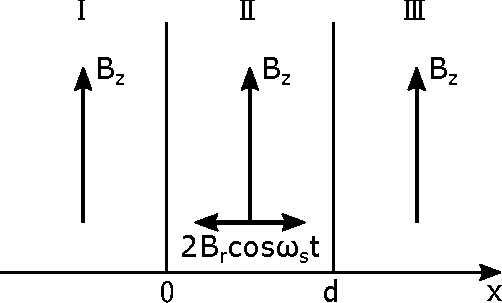
\includegraphics[height=3cm]{resonance/whatwhyhow/Resonance_what_setting.pdf}
\end{figure}

\ref{nonreso_sec}章で述べたように、領域Iからスピン上向きの中性子を入射したとき領域IIIでスピン上向きの中性子を観測する確率は
\begin{equation}
|\psi_{\mathrm{III}}^+|^2=\cos^2 \frac{\omega_A}{v}d+\left(\frac{\epsilon}{\omega_A}\right)^2\sin^2\frac{\omega_A}{v}d \label{Resonance_flip}
\end{equation}
となる。ここで$\epsilon=\omega_s/2-\omega_z,\omega_A=\sqrt{\epsilon^2+\omega_r^2}$であり、$\omega_z=|\mu_n|B_z,\omega_r=|\mu_n|B_r$、$\mu_n$は中性子の磁気モーメント、$d$は領域IIの幅である。

いま$\epsilon/|\omega_z|=0,0.3,0.5,1.0$の各場合についてスピンフリッパーを通過した中性子のスピン反転率($=1-|\psi_\mathrm{III}^+|^2$)と$\omega_r d/v$の関係を図\ref{Resonance_fig_reversalrate}に表す。
図\ref{Resonance_fig_reversalrate}より
\begin{equation}
\epsilon=\frac{\omega_s}{2}-\omega_z=0 \label{Resonance_resonance}
\end{equation}
がなりたてば、
\begin{equation}
\frac{\omega_r}{v}d =\frac{(2n+1)\pi}{2} \quad (n =0,1,2,\cdots) \label{Resonance_piflip_r}
\end{equation}
を満たす速度の中性子に対して、領域IIIにおけるスピン上向き粒子の存在確率が0、すなわちスピン反転率が1になることがわかる。逆に$\epsilon \neq 0$のときはどのような速度の中性子に対しても反転率は1となり得ない。このように、式(\ref{Resonance_resonance})を満たす周波数の振動磁場をかけたときに限りスピンフリッパーを通り抜けた中性子のスピンが完全に反転し得る。これをスピンフリッパーの共鳴と呼び、式(\ref{Resonance_resonance})を共鳴条件と呼ぶ。また速度に対する条件(\ref{Resonance_piflip_r})を$\pi$フリップ条件と呼ぶ。
\begin{figure}[h]
\begin{center}
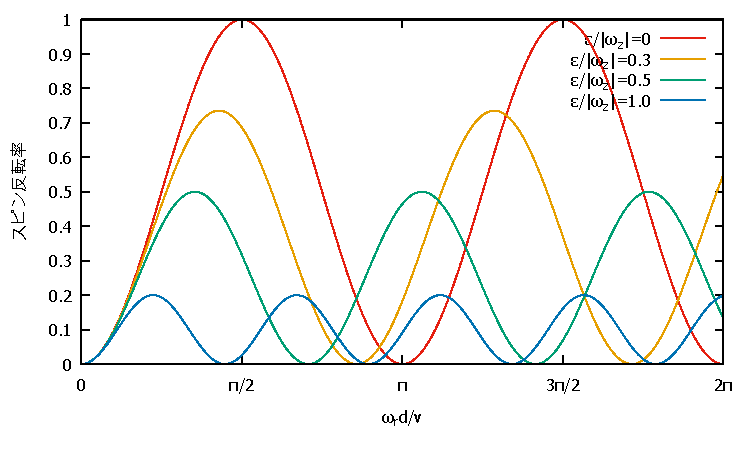
\includegraphics[width=9.5cm]{resonance/whatwhyhow/resonance_reversalrate.pdf}
\caption{スピン反転率}
\label{Resonance_fig_reversalrate}
\end{center}
\vspace{-1cm}
\end{figure}

\subsection{Why?\ $\sim$スピンフリッパーの共鳴はなぜ必要か$\sim$}
スピンフリッパーの共鳴は本実験での干渉がはっきり見えるかどうかの鍵を握っている。ここではスピンフリッパー共鳴の重要性が明らかとなる。

一様磁場中に、理想化されたRFスピンフリッパーふたつとシフタコイルひとつが置かれた状況を考える。系は7つの領域I,II,III,IV,V,VI,VIIからなり、全体に$z$方向一様磁場$B_z$がかけられ、それに加えて領域II,VIに$x$方向振動磁場$2B_r\cos\omega_s t$が、領域IVに$z$方向一様磁場$B$がかけられている。
\begin{figure}[h]
\centering
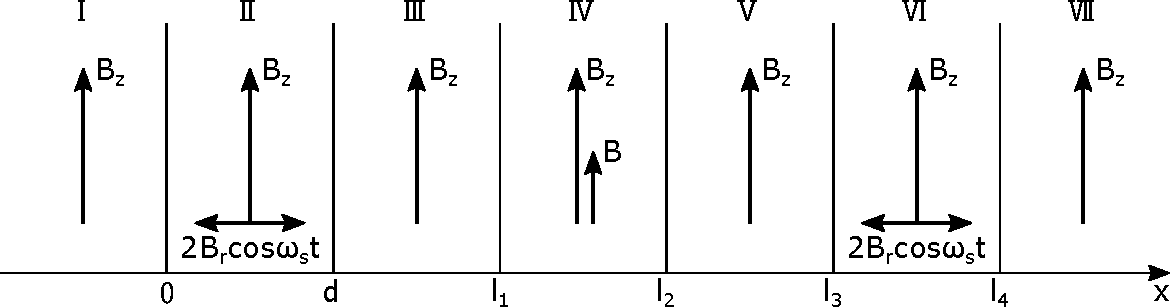
\includegraphics[height=3cm]{resonance/whatwhyhow/Resonance_why_setting.pdf}
\end{figure}

\ref{nonreso_sec}章で述べたように、スピン上向きの中性子が領域Iから入射し、領域I$\sim$VIを通って領域VIIに抜けるとき、領域VIIにおいてスピン上向き中性子を観測する確率は、共鳴からのずれを表すパラメータ$\epsilon$と中性子の速度$v$に依存した係数$N_1,N_2,N_3$を用いて
\begin{equation}
I=N_1-N_2\cos\left(\frac{2}{v}(\omega d'-\epsilon L')\right) -N_3\sin\left(\frac{2}{v}(\omega d'-\epsilon L')\right) \label{analysis_theory_ippan}
\end{equation}
と表せる。ここで$\omega$は位相シフタコイルの磁場$B$を用いて$\omega=|\mu_n|B$と表される量であり、$d',L'$はそれぞれ位相シフタコイルの幅、2つのスピンフリッパー間距離である。さらに$N_4=\sqrt{N_2^2+N_3^2}$として
\begin{equation}
\cos \phi=\frac{N_2}{N_4}, \quad \sin \phi=\frac{N_3}{N_4}
\end{equation}
で$\phi$を定義すれば、干渉パターンは
\begin{equation}
I=N_1-N_4\cos\left(\frac{2}{v}(\omega d'-\epsilon L')-\phi\right)\label{Resonance_interference}
\end{equation}
と書き直される。

いま、ある$\epsilon$に対して、シフタコイルの磁場を変えながら領域VIIでのスピン上向き中性子の数を計測すると式(\ref{Resonance_interference})の干渉パターンが得られるが、その見えやすさ(ビジビリティ)は$\epsilon$によって異なる。例えば$N_4/N1=1$のときは振幅の大きなはっきりとした(ビジビリティの高い)干渉パターンが得られるが、$N_4/N_1 \ll 1$のときは干渉パターンはほとんど観測できない(ビジビリティが低い)。そこでビジビリティを表す指標$V$を
\begin{equation}
V=\frac{N_4}{N_1}
\end{equation}
で定義すると、$0 \le V \le 1$であり、$V$が大きい程ビジビリティが高い。

いま$\epsilon/|\omega_z|=0,0.3,0.5,1.0$の各場合について干渉パターンのビジビリティ$V$と$\omega_r d/v$の関係を図\ref{Resonance_fig_visivility}に表す。図\ref{Resonance_fig_visivility}より共鳴条件(\ref{Resonance_resonance})がなりたてば、
\begin{equation}
\frac{\omega_r }{v}d =\frac{(2n+1)\pi}{4} \quad (n =0,1,2,\cdots) \label{Resonance_pi2flip_r}
\end{equation}
を満たす速度の中性子に対して、干渉パターンのビジビリティ$V=1$になることがわかる。逆に$\epsilon \neq 0$のときはどのような速度の中性子に対してもビジビリティは1となり得ない。この速度に対する条件(\ref{Resonance_pi2flip_r})を$\pi/2$フリップ条件と呼ぶ。実際、$\omega_rd/v=\pi/4$,$\epsilon/|\omega_z|=0,0.3,0.5,1.0$のときの干渉パターンは図\ref{Resonance_fig_interference}のようになる。すなわちスピンフリッパーを共鳴させる目的は、本実験で得られる干渉パターンのビジビリティを高めるためである。

\begin{figure}[h]
\vspace{-2mm}
\begin{center}
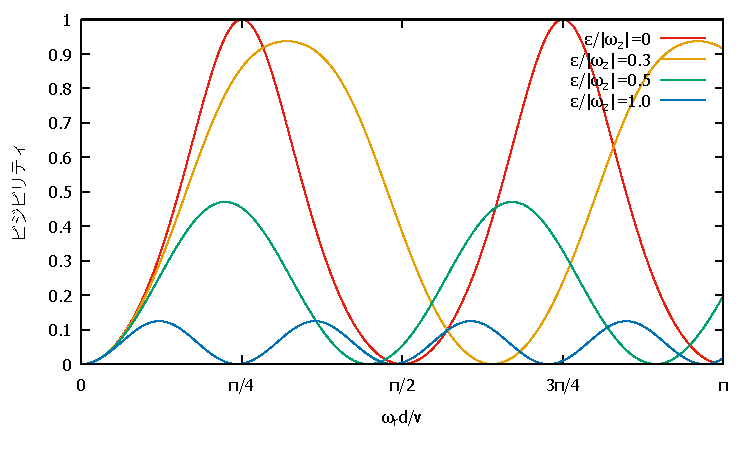
\includegraphics[width=9.5cm]{resonance/whatwhyhow/resonance_visivility1.pdf}
\caption{ビジビリティ}
\label{Resonance_fig_visivility}
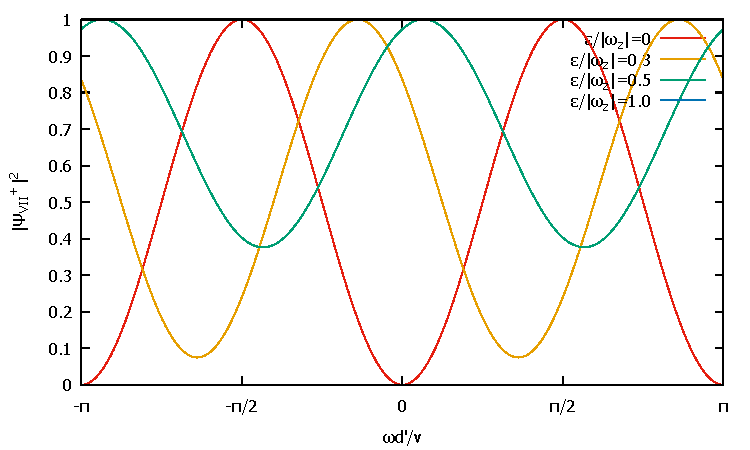
\includegraphics[width=9.5cm]{resonance/whatwhyhow/resonance_interference1.pdf}
\caption{干渉パターン}
\label{Resonance_fig_interference}
\end{center}
\vspace{-1cm}
\end{figure}



\clearpage
\subsection{How?\ $\sim$スピンフリッパーを共鳴させるには$\sim$}
実際にスピンフリッパーを共鳴させるにはどうしたらよいだろう。ここではその実現方法を考え、実際に実験で用いた装置と従った手順を紹介する。

\paragraph{実現方法}
\ref{Resonance_what}節と同じく、一様磁場中にスピンフリッパーがひとつ置かれており、スピン上向き中性子を領域Iから入射させる場合を考える。このとき領域IIIでスピン上向き中性子を観測する確率は式(\ref{Resonance_flip})より
\begin{equation}
|\psi_\mathrm{III}^+|^2 =\cos^2 \frac{\omega_A}{v}d+\left(\frac{\epsilon}{\omega_A}\right)^2\sin^2\frac{\omega_A}{v}d
\end{equation}
であらわされる。これを$\omega_r/|\omega_z|=0.5$のときに、$\epsilon/|\omega_z|=0,0.3,0.5,1.0$の各場合について$\omega_r d/v$に対して図示すると図\ref{Resonance_fig_1-reversal}のようになる。図\ref{Resonance_fig_1-reversal}より、領域IIIでスピン上向き中性子を観測する確率の、速度に対する最小値は共鳴条件(\ref{Resonance_resonance})
を満たすとき最も小さくなり、理想的にはゼロとなることがわかる。共鳴条件を満たすときにスピンフリッパーを通り抜けた中性子のスピン反転率が$1,1/2$となるための中性子の速度に対する条件をそれぞれ$\pi$フリップ条件(\ref{Resonance_piflip})、$\pi/2$フリップ条件(\ref{Resonance_pi2flip})と呼んだが、今回の実験で用いた中性子の速度範囲ではそれぞれ$n=0$の場合のみが満たされ得るので、以後
\begin{equation}
\frac{\omega_r}{v}d=\frac{\pi}{2}\label{Resonance_piflip}
\end{equation}
を$\pi$フリップ条件
\begin{equation}
\frac{\omega_r}{v}d=\frac{\pi}{4}\label{Resonance_pi2flip}
\end{equation}
を$\pi/2$フリップ条件と呼ぶことにする。
\begin{figure}[h]
\begin{center}
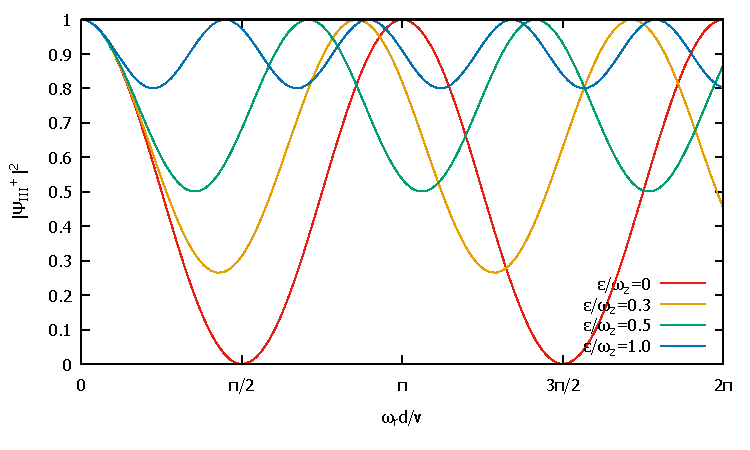
\includegraphics[width=9.5cm]{resonance/whatwhyhow/resonance_1-reversal.pdf}
\caption{$1-反転率$}
\label{Resonance_fig_1-reversal}
\end{center}
\end{figure}

すなわち次のようにして、実験的にスピンフリッパーの共鳴を実現することができる。
\begin{enumerate}
\item スピンフリッパーにスピン上向き中性子を入射し、フリッパーの後ろでスピン上向き成分のみを観測する。
\item 共鳴条件(\ref{Resonance_resonance})が満たされていないと、ある速度の中性子についてはカウントをより減らすことができる。
\item 共鳴条件(\ref{Resonance_resonance})が満たされていると、$\pi$フリップ条件(\ref{Resonance_piflip})を満たす速度の中性子についてはスピンが完全に反転するため、その速度の中性子のカウントは最小となる。
\item カウント分布を見ながら共鳴条件(\ref{Resonance_resonance})に関するパラメータを調節し、カウントが最小となるところを探す。
\end{enumerate}


\paragraph{実験装置}
上流側、下流側それぞれのスピンフリッパーに対して共鳴実験を行った。用いた装置は
\vspace{5mm}
\begin{minipage}{0.5\hsize}
\begin{enumerate}
\item 上流側スピンフリッパー共鳴実験
\begin{enumerate}
\item ガイド磁場コイル
\item 上流側中性子磁気スーパーミラー
\item[(c1)] 上流側スピンフリッパー
\setcounter{enumii}{3}
\item 下流側中性子磁気スーパーミラー
\item \ce{^3He}ガスを充填した比例計数管
\end{enumerate}
\end{enumerate}
\end{minipage}
\begin{minipage}{0.5\hsize}
\begin{enumerate}
\setcounter{enumi}{1}
%\renewcommand{\labelenumi}{}
\item 下流側スピンフリッパー共鳴実験
\begin{enumerate}
\item ガイド磁場コイル
\item 上流側中性子磁気スーパーミラー
%\renewcommand{\labelenumi}{(\alph{enumi} {2})}
\item[(c2)] 下流側スピンフリッパー
\setcounter{enumii}{3}
%\renewcommand{\labelenumi}{(\alph{enumi})}
\item 下流側中性子磁気スーパーミラー
\item \ce{^3He}ガスを充填した比例計数管
\end{enumerate}
\end{enumerate}
\end{minipage}
\vspace{5mm}

また、回路系には次の機器を用い、図のように接続した。
\begin{enumerate}
\renewcommand{\labelenumi}{(\roman{enumi})}
\item 直流安定化電源PWX750MLF(KIKUSUI) $\times 3$ \ \ (以後、直流電源1,2,3)
\item マルチファンクションジェネレータWF1974(エヌエフ回路設計ブロック) \ \ (以後、FG)
\item 1MHzバイポーラ電源HSA4014(エヌエフ回路設計ブロック) $\times 2$ \ \ (以後、アンプ1,2)
\end{enumerate}

\vspace{5mm}
\begin{figure}[h]
\centering
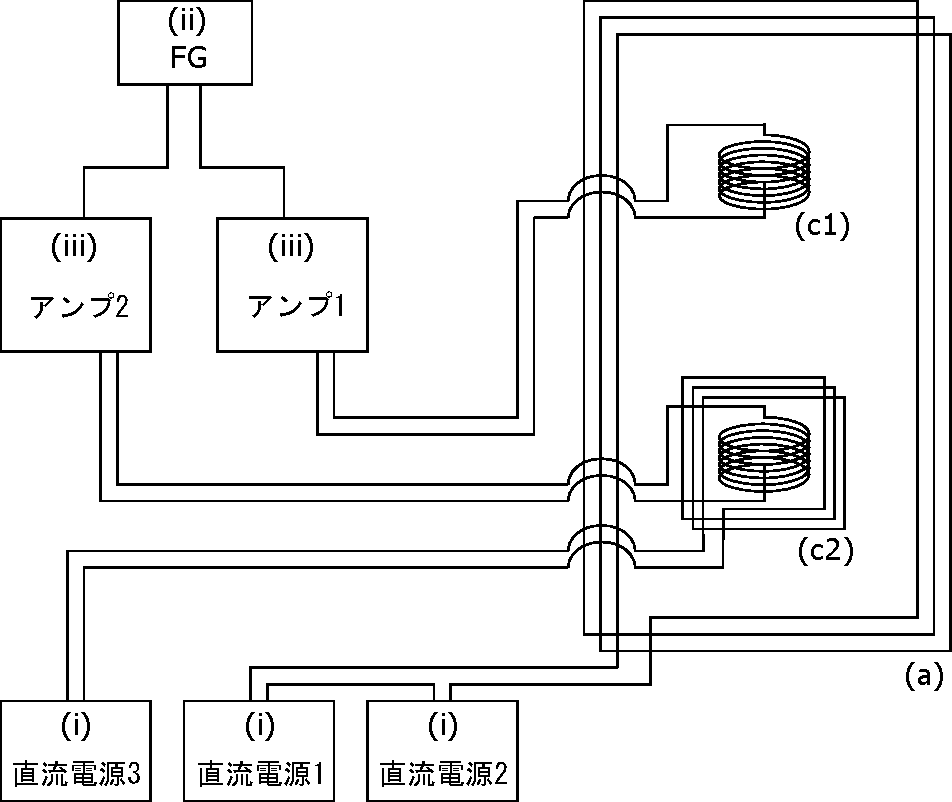
\includegraphics[width=12cm]{resonance/whatwhyhow/kairozu.pdf}
\caption{配線図}
\vspace{-5mm}
\end{figure}

\clearpage
\paragraph{実験手順}
実験は次のフローチャートに沿って行った。
\begin{figure}[h]
\centering
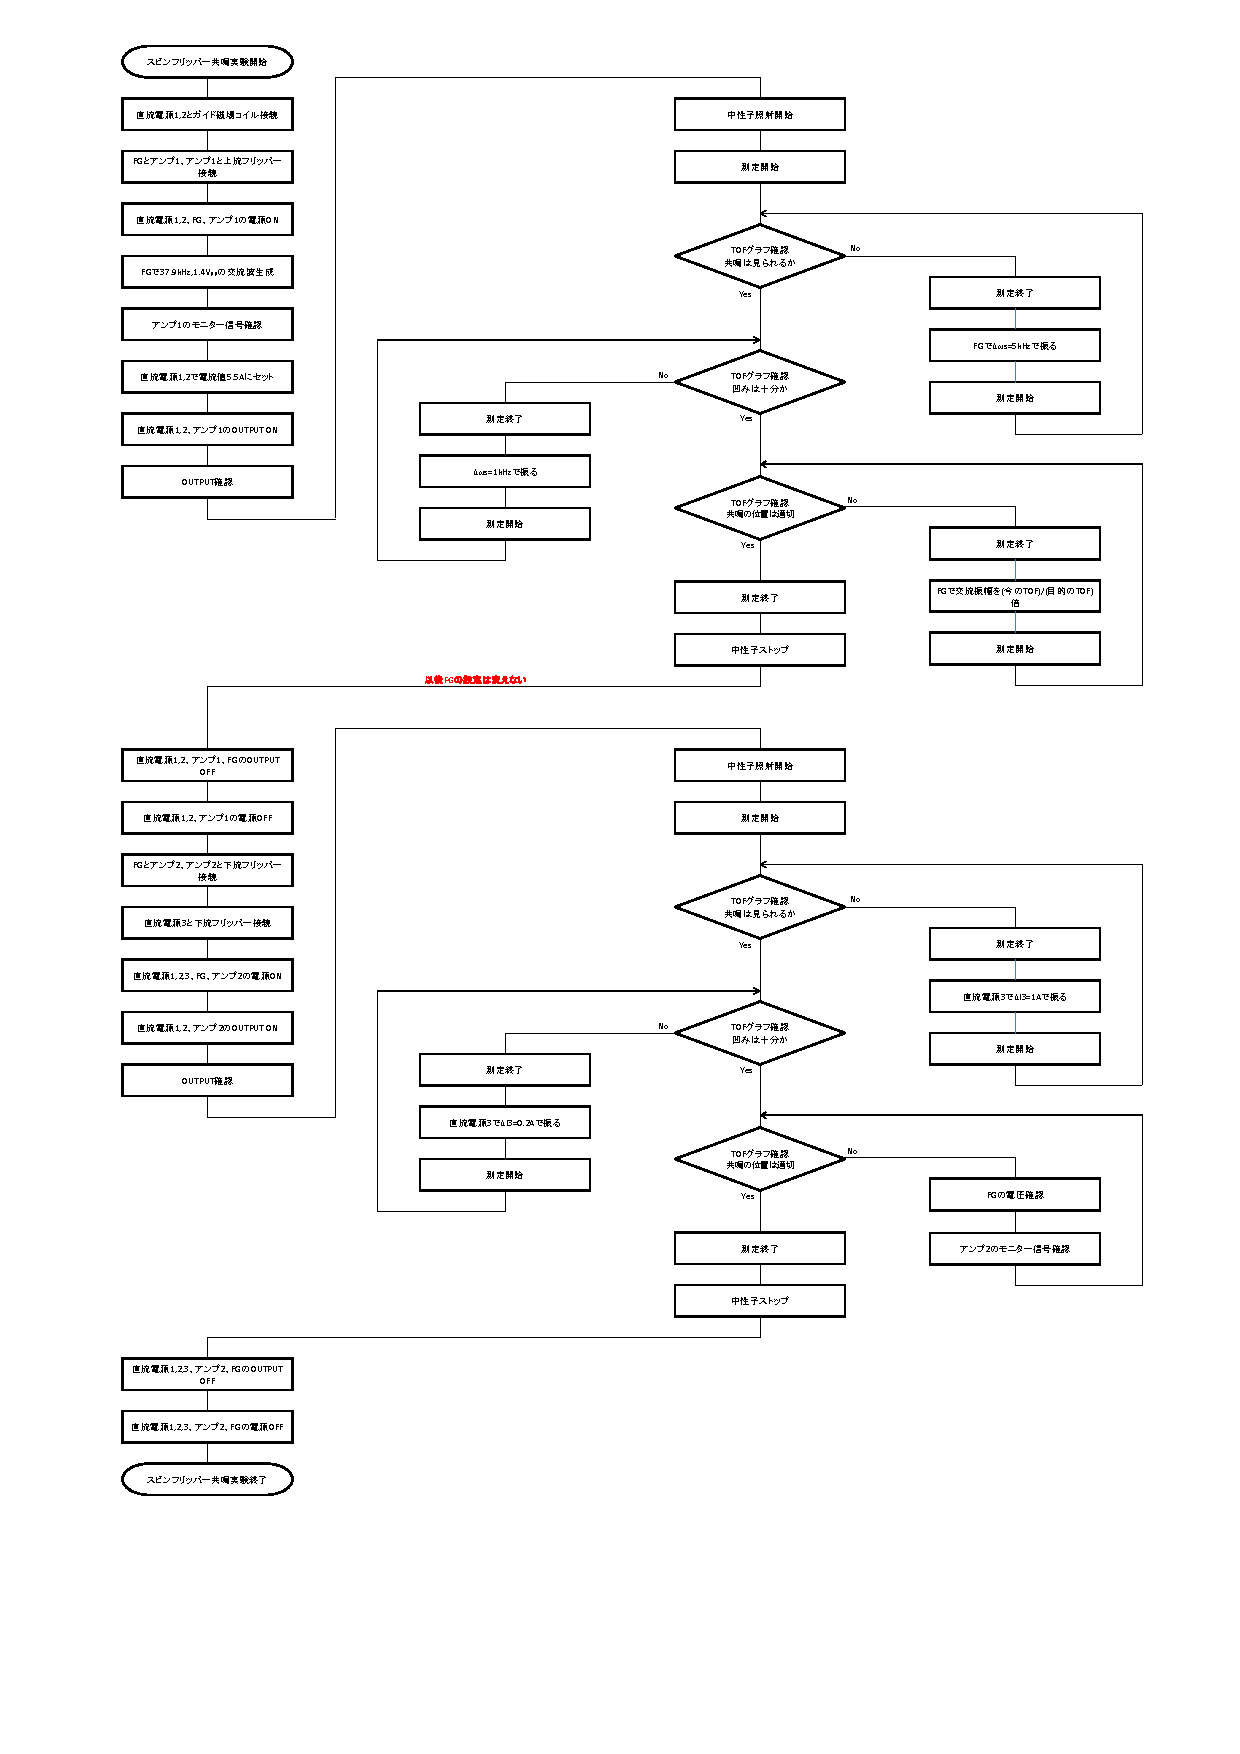
\includegraphics[width=\hsize]{resonance/whatwhyhow/Resonance_flow.pdf}
\vspace{-3.5cm}
\end{figure}

\newpage
次は実際の実験手順である。
\begin{enumerate}
%\renewcommand{\labelenumi}{\arabic{enumi})}
\item (2017.2.22)装置、機器を図のとおりに配置、接続し、上流フリッパー共鳴実験を開始した。
\item 直流電源1,2でガイド磁場コイルに5.5Aの電流を流した。
\item FGで周波数$37.9\, \mathrm{kHz},振幅14.0\, \mathrm{V_{pp}}$の交流波を生成し、アンプ1で増幅して上流フリッパーに交流電流を流した。
\item 中性子の照射を開始した。
\item 測定を開始した。
\item 10分程度データを取り、TOF分布に凹みを確認した。
\item FGで交流波の周波数を$37.0,38.8,36.0,34.0,41.0,40.0 \, \mathrm{kHz}$と変えながら、それぞれ10分程度データを収集した。
\item データ収集と平行して解析を行い、交流波の周波数を$37.5\, \mathrm{kHz}$,振幅を$14.0\, \mathrm{V_{pp}}$に決定した。
\item 中性子照射をストップし、機器の電源を落として上流フリッパー共鳴実験を終了した。
\item (2017.2.23)装置、機器を図のとおりに配置、接続し、下流フリッパー共鳴実験を開始した。
\item 直流電源1,2でガイド磁場コイルに5.5Aの電流を流した。
\item FGで周波数$37.5\, \mathrm{kHz},振幅14.0\, \mathrm{V_{pp}}$の交流波を生成し、アンプ2で増幅して下流フリッパーに交流電流を流した。
\item 中性子の照射を開始した。
\item 測定を開始した。
\item 10分程度データを取り、TOF分布に凹みを確認した。
\item 直流電源3でガイド磁場補正用コイルに流す電流を$0.1,0.5,0.3,0.7\,\mathrm{A}$と変えながら、それぞれ10分程度データを収集した。
\item 一旦中性子照射をストップし直流電源3をガイド磁場補正用コイルに逆向きにつなぎ替え、再び中性子照射を開始した。
\item 直流電源3でガイド磁場補正用コイルに流す電流を$-1.0,-0.5,-2.0\,\mathrm{A}$と変えながら、それぞれ10分程度データを収集した。
\item 一旦中性子照射をストップし直流電源3をガイド磁場補正用コイルに逆向きにつなぎ替え、再び中性子照射を開始した。
\item 直流電源3でガイド磁場補正用コイルに流す電流を$1.0,2.0\,\mathrm{A}$と変えて、それぞれ10分程度データを収集した。
\item データ収集と平行して解析を行い、ガイド磁場補正用コイルの電流値を$0.185\,\mathrm{A}$に決定した。
\item 中性子照射をストップし、機器の電源を落として下流フリッパー共鳴実験を終了した。
\end{enumerate}

\begin{itemize}
\item[(注$\!\!$1)] ガイド磁場コイル、ガイド磁場補正用コイルに流す電流は、電流を流したときに鉛直下向きの磁場が発生する向きを正とした。
\item[(注$\!\!$2)] 下流フリッパー共鳴実験中、ガイド磁場コイルが接触不良のためうまく機能せず正しいデータが取れない事態が発生したが、それについては省略した。
\end{itemize}

%\newpage
\paragraph{パラメータ初期設定}
スピンフリッパー共鳴実験で実際に制御できるパラメータはFGで生成する交流電圧の周波数$f_s$,振幅$V_r$と直流電源3で下流フリッパーのガイド磁場補正用コイルに流す電流$I_c$の3つである。実験は共鳴条件(\ref{Resonance_resonance})と$\pi$フリップ条件(\ref{Resonance_piflip})を満たすようにこれらを適当に変えながら進めたが、初期設定としてこれらの値をある程度正確に決めておく必要がある。なぜなら、もし最初に全く共鳴が見えないと、どのパラメータをどの程度動かしてよいか全く見当がつかないから。

スピンフリッパーにかける振動磁場の角振動数$\omega_s$と振幅$2B_r$の2つのは、それぞれフリッパーが置かれた場所におけるガイド磁場コイルの磁場$B_z$とターゲットとする中性子の速度$v$から定まる。すなわち$\omega_s$は共鳴条件(\ref{Resonance_resonance})より
\begin{equation}
\omega_s = 2\omega_z =2 |\mu_n|B_z
\end{equation}
$B_r$は$\pi$フリップ条件(\ref{Resonance_piflip})より
\begin{equation}
2B_r =\frac{2 \omega_r}{|\mu_n|} =\frac{\pi v}{|\mu_n|d}
\end{equation}
で定まる。

$B_z$としてはシミュレーションと実測より$B_z=-13 \, \mathrm{G}$を、$v$としてはフリッパー無しのときの速度分布である程度カウントの多かった$v=1000\, \mathrm{m/s}$を入れてそれぞれ計算すると
\begin{equation}
|\omega_s|/2\pi\simeq 37.9\, \mathrm{kHz}, \quad B_r\simeq 5.7 \, \mathrm{G}
\end{equation}
を得る。従ってFGで生成する交流電圧の周波数$f_s$の初期値は$37.9\,\mathrm{kHz}$と決めた。

また、フリッパーを直径90mm幅30mmの30巻きソレノイドコイルとして、1Aの電流を流したときの中心での磁場の大きさ$b_f$[G]と、37.9kHzの交流電圧をかけたときのインピーダンス$Z[\Omega]$を計算するとそれぞれ
\begin{equation}
b_f\simeq 3.9 \,\mathrm{G} \qquad Z \simeq 24.5 \,\Omega
\end{equation}
となる。ゆえにフリッパーにかける交流電圧の振幅(peak to peak)は
\[2 \times \frac{2B_r}{b_f} \times Z \simeq 140 \mathrm{V_{pp}}\]
となる。アンプで振幅を約100倍にすることを考えて、FGで生成する交流電圧の振幅$V_r$の初期値は$1.4 \,\mathrm{V_{pp}}$と決めた。

また、シミュレーションと実測よりガイド磁場の大きさは上流フリッパーの位置と下流フリッパーの位置でほぼ等しいことがわかっていたため、フリッパーのガイド磁場補正用コイルに流す電流の$I_c$の初期値は$0\,\mathrm{A}$と決めた。

まとめると
\begin{table}[h]
\centering
\caption{パラメータ初期値}
\begin{tabular}{ccc}
$f_s$の初期値&$V_r$の初期値&$I_c$の初期値 \\ \hline
$37.9\,\mathrm{kHz}$&$1.4 \,\mathrm{V_{pp}}$&$0\,\mathrm{A}$
\end{tabular}
\end{table}

\subsection{測定データ}
実際に共鳴実験で得られたデータを以下に示す。上流フリッパー共鳴実験で周波数を$|\omega_s|/2\pi=34.0,36.0,37.0,37.9,38.8,40.0,41.0$kHzと変えたとき、それぞれの場合に得られた粒子数の波長分布を図\ref{Resonance_fig_Flipper1_RawCounts}に、下流フリッパー共鳴実験でガイド磁場補正用コイル電流を$I_c=-2.0,-1.0,-0.5,0,0.1,0.3,0.5,1.0,2.0$Aと変えたとき、それぞれの場合に得られた粒子数の波長分布を図\ref{Resonance_fig_Flipper2_RawCounts}に表す。

\begin{figure}[h]
%\begin{minipage}{0.49\hsize}
%\centering
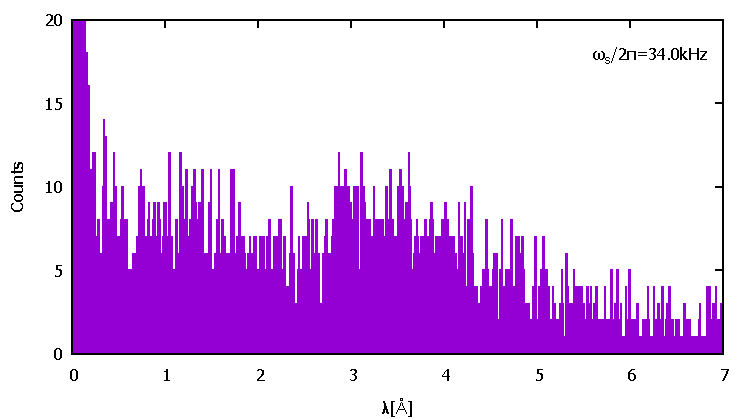
\includegraphics[height=4.3cm]{resonance/results/Flipper1_RawCounts_340kHz.pdf}
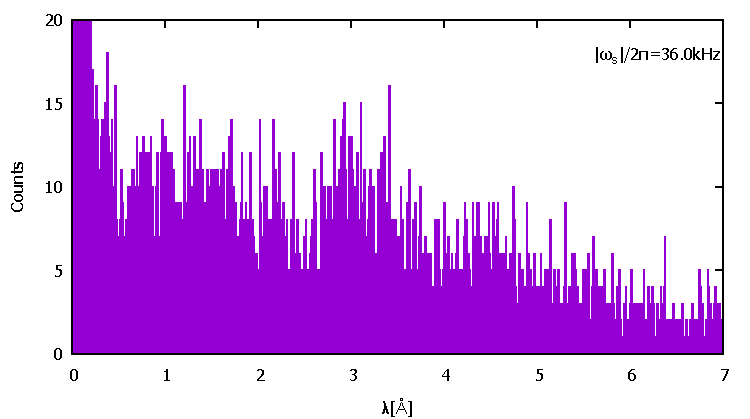
\includegraphics[height=4.3cm]{resonance/results/Flipper1_RawCounts_360kHz.pdf}\\
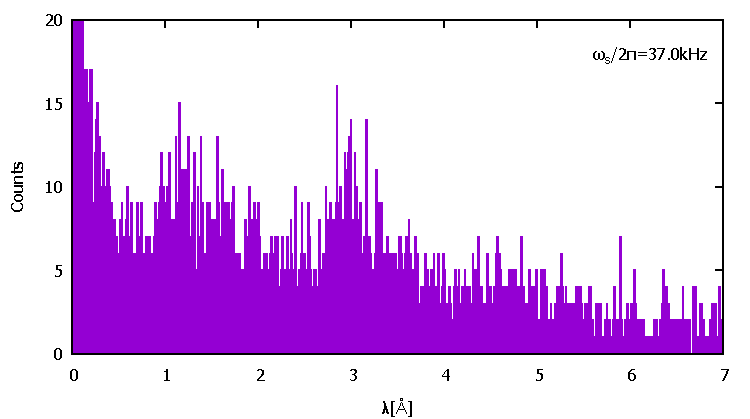
\includegraphics[height=4.3cm]{resonance/results/Flipper1_RawCounts_370kHz.pdf}
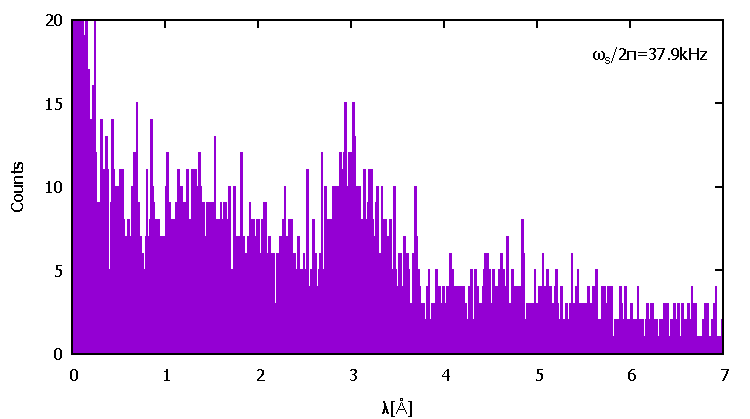
\includegraphics[height=4.3cm]{resonance/results/Flipper1_RawCounts_379kHz.pdf}\\
%\end{minipage}
%\begin{minipage}{0.49\hsize}
%\centering
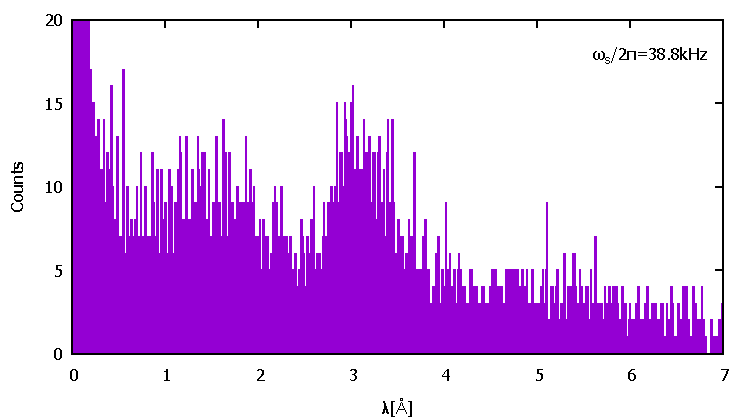
\includegraphics[height=4.3cm]{resonance/results/Flipper1_RawCounts_388kHz.pdf}
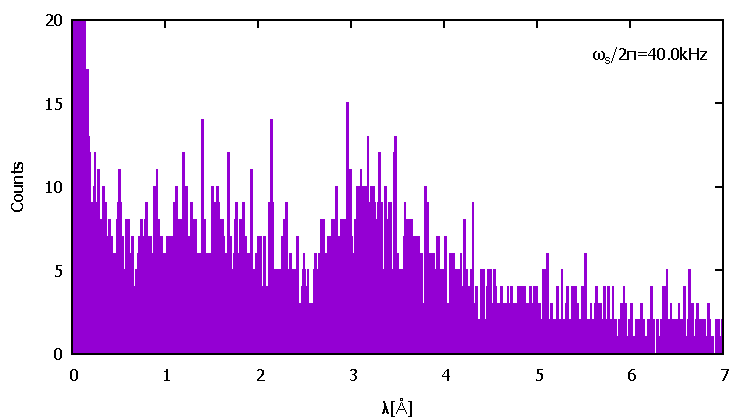
\includegraphics[height=4.3cm]{resonance/results/Flipper1_RawCounts_400kHz.pdf}\\
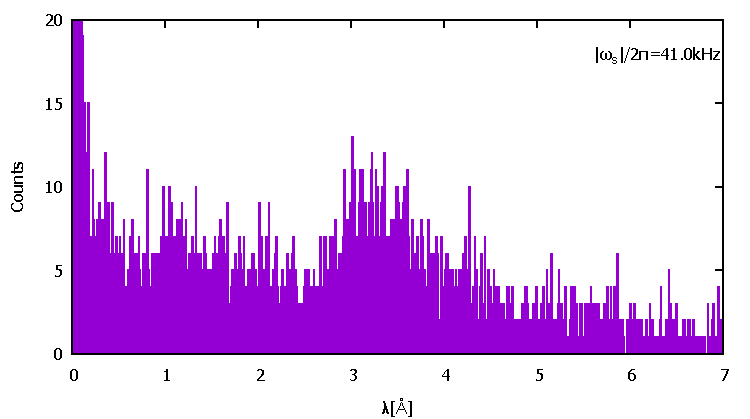
\includegraphics[height=4.3cm]{resonance/results/Flipper1_RawCounts_410kHz.pdf}
%\vspace{4.3cm}
%\end{minipage}
\caption{上流フリッパー共鳴実験で得られた粒子数の波長分布}\label{Resonance_fig_Flipper1_RawCounts}
\end{figure}

\begin{figure}[h]
%\begin{minipage}{0.5\hsize}
%\centering
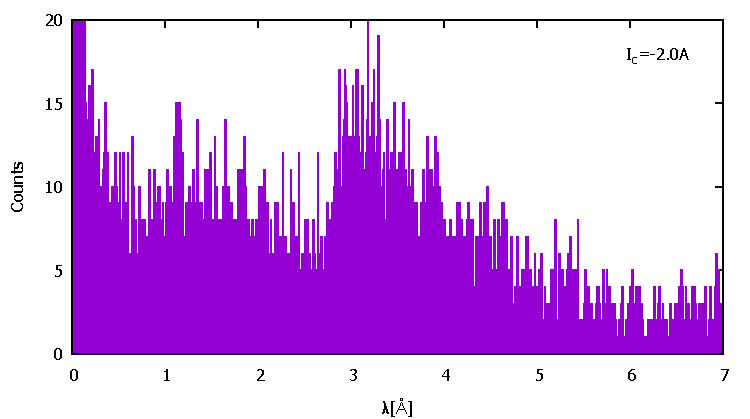
\includegraphics[height=4.3cm]{resonance/results/Flipper2_RawCounts_-20A.pdf}
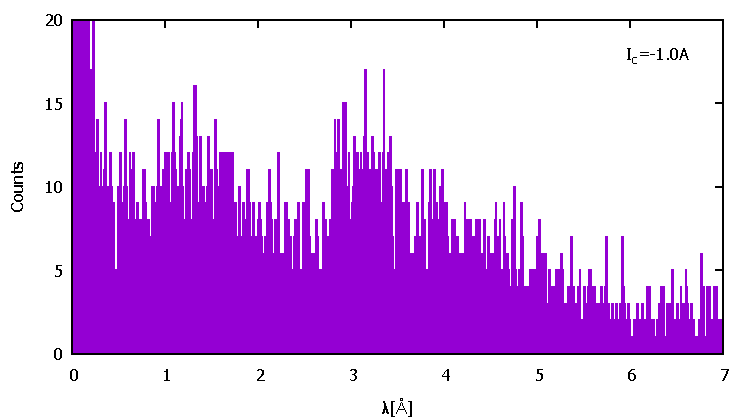
\includegraphics[height=4.3cm]{resonance/results/Flipper2_RawCounts_-10A.pdf}\\
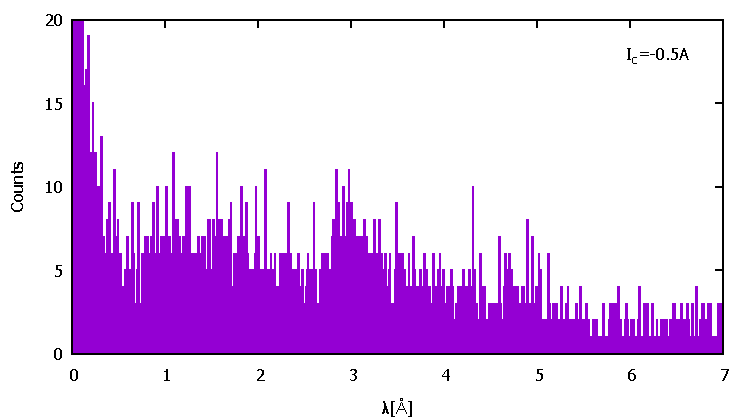
\includegraphics[height=4.3cm]{resonance/results/Flipper2_RawCounts_-5A.pdf}
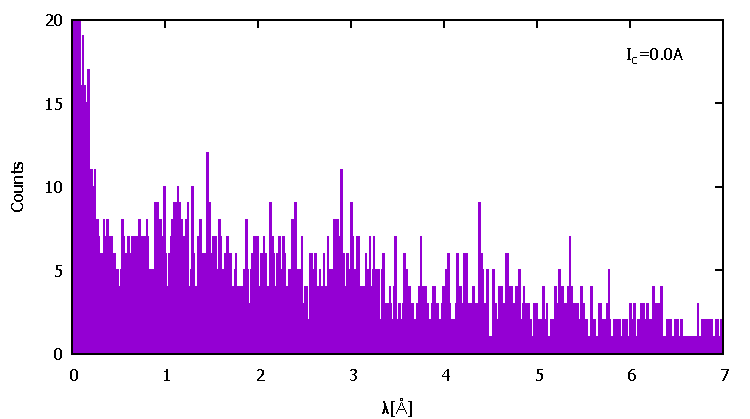
\includegraphics[height=4.3cm]{resonance/results/Flipper2_RawCounts_0A.pdf}\\
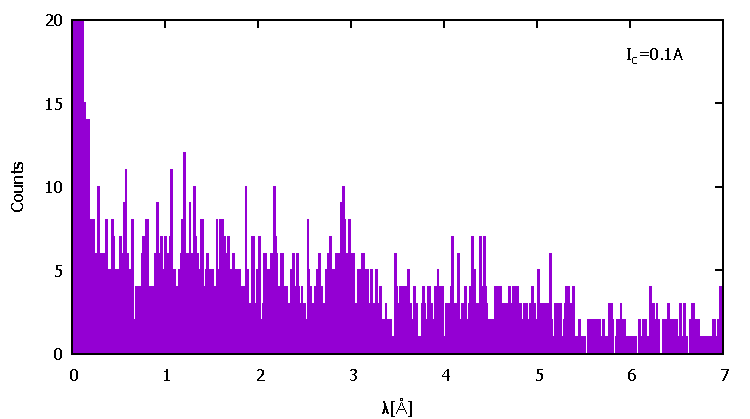
\includegraphics[height=4.3cm]{resonance/results/Flipper2_RawCounts_1A.pdf}
%\end{minipage}
%\begin{minipage}{0.5\hsize}
%\centering
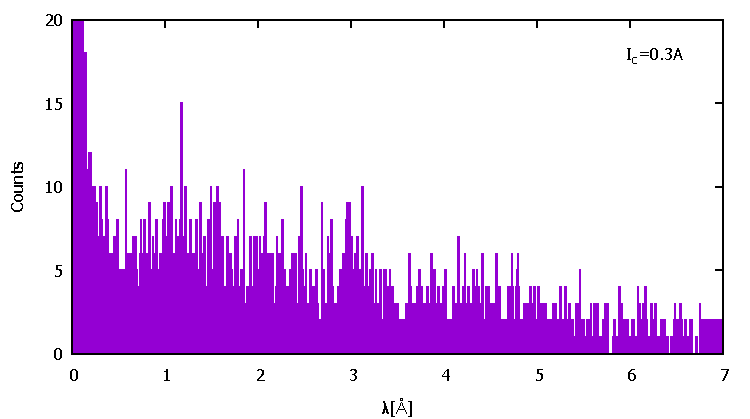
\includegraphics[height=4.3cm]{resonance/results/Flipper2_RawCounts_3A.pdf}\\
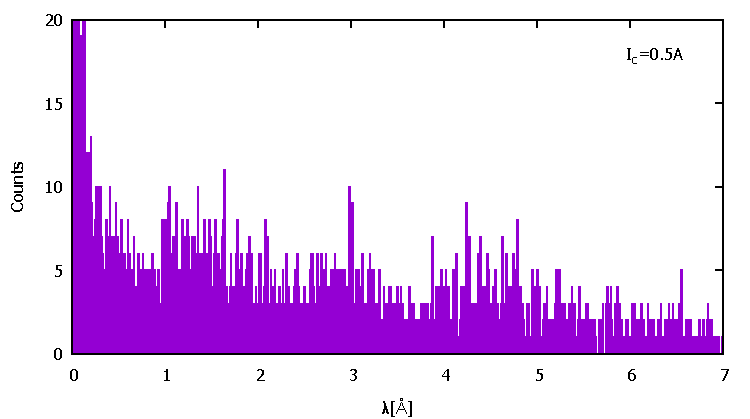
\includegraphics[height=4.3cm]{resonance/results/Flipper2_RawCounts_5A.pdf}
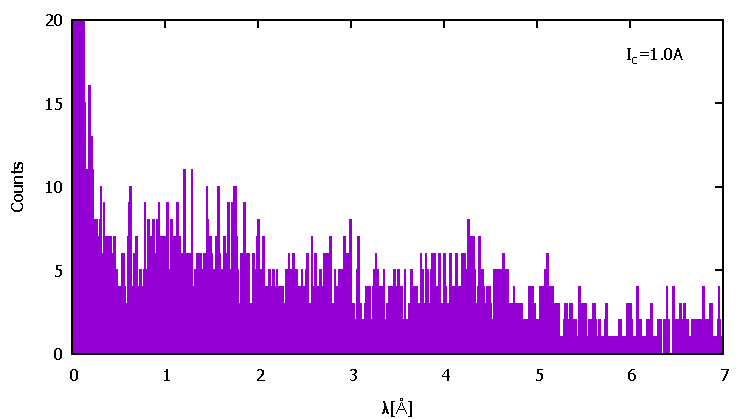
\includegraphics[height=4.3cm]{resonance/results/Flipper2_RawCounts_10A.pdf}\\
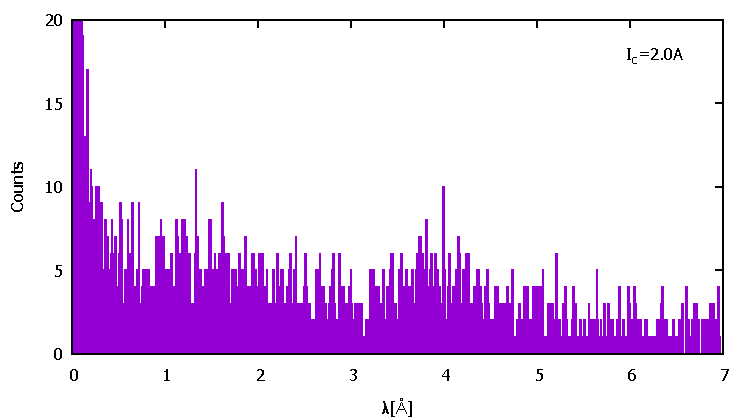
\includegraphics[height=4.3cm]{resonance/results/Flipper2_RawCounts_20A.pdf}
%\vspace{4.3cm}
%\end{minipage}
\caption{下流フリッパー共鳴実験で得られた粒子数の波長分布}\label{Resonance_fig_Flipper2_RawCounts}
\end{figure}

\clearpage
\subsection{分析}
以下では
\begin{enumerate}
\item 上流フリッパーについてデータから共鳴条件(\ref{Resonance_resonance})を満たす$\omega_s$を決め、グラフから共鳴時に最もよくスピン反転する中性子の波長を推定し、$\pi$フリップ条件(\ref{Resonance_piflip})から$\omega_r$を計算する。
\item 上流フリッパーについてデータから共鳴条件(\ref{Resonance_resonance})を満たす$I_c$を決め、グラフから共鳴時に最もよくスピン反転する中性子の波長を推定し、$\pi$フリップ条件(\ref{Resonance_piflip})から$\omega_r$を計算する。
\end{enumerate}
という流れでデータの分析を行う。

\paragraph{上流フリッパーに関する分析}
共鳴しているかを知るにはパラメータを変えたときの検出粒子数を比較すればよく、ある波長でカウントが最小となるとき共鳴していると考えてよい。しかし前節で示したデータは測定時間や加速器の出力がそれぞれ異なるので、そのままでは互いに比較することができない。そこで測定データのカウントをそのデータの測定開始時刻から測定終了時刻までにおけるLiMのカウントで割って規格化することで、データを互いに比較できるようにする。このようにして規格化した上流フリッパー共鳴実験における粒子数の波長分布を、フリッパーをOFFにしたときの規格化粒子数と共に、図\ref{Resonance_fig_Flipper1_NormalizedCounts}に表す。

\begin{figure}[h]
%\begin{minipage}{0.49\hsize}
%\centering
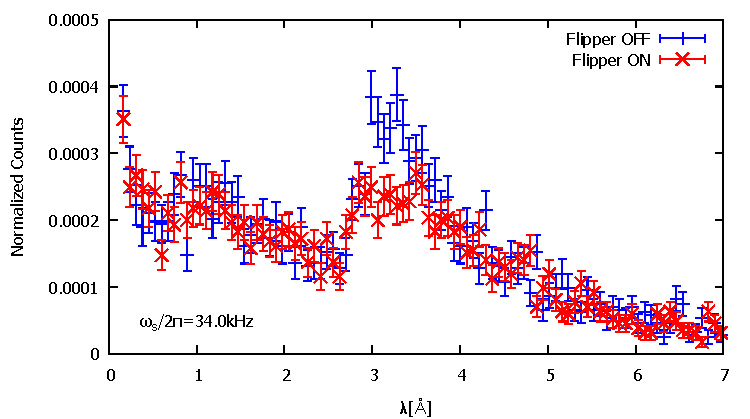
\includegraphics[height=4.3cm]{resonance/analysis/Flipper1_NormalizedCounts_340kHz.pdf}
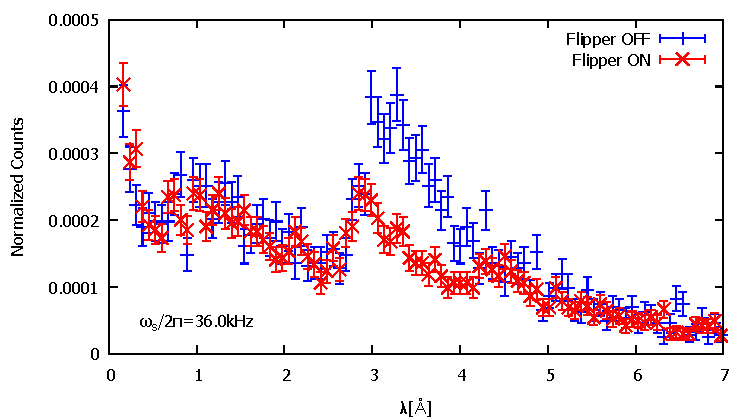
\includegraphics[height=4.3cm]{resonance/analysis/Flipper1_NormalizedCounts_360kHz.pdf}\\
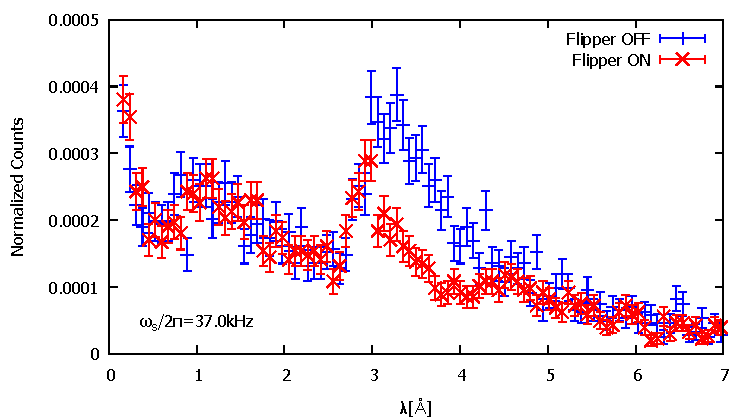
\includegraphics[height=4.3cm]{resonance/analysis/Flipper1_NormalizedCounts_370kHz.pdf}
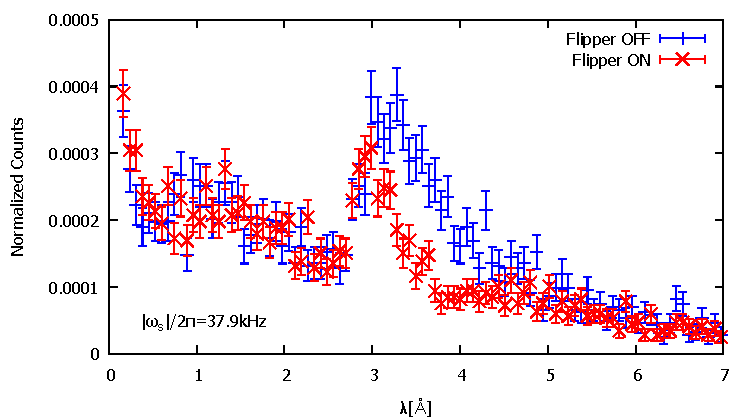
\includegraphics[height=4.3cm]{resonance/analysis/Flipper1_NormalizedCounts_379kHz.pdf}\\
%\end{minipage}
%\begin{minipage}{0.49\hsize}
%\centering
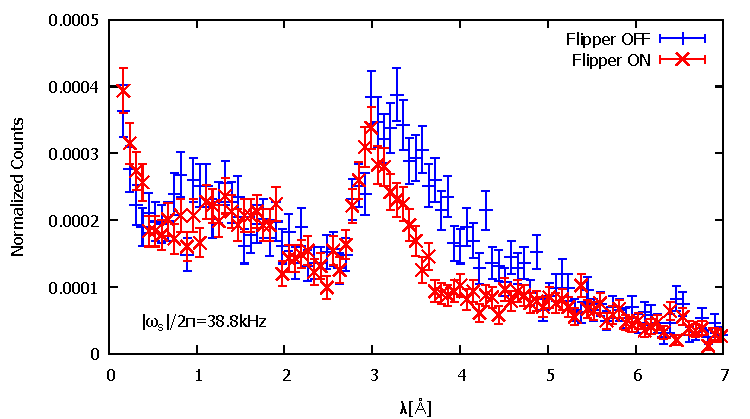
\includegraphics[height=4.3cm]{resonance/analysis/Flipper1_NormalizedCounts_388kHz.pdf}
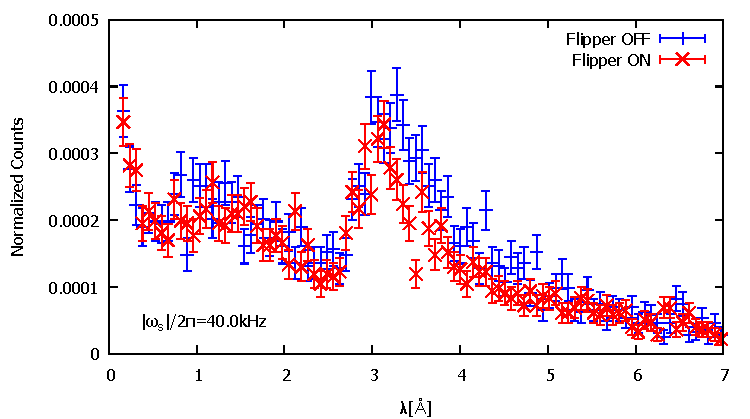
\includegraphics[height=4.3cm]{resonance/analysis/Flipper1_NormalizedCounts_400kHz.pdf}\\
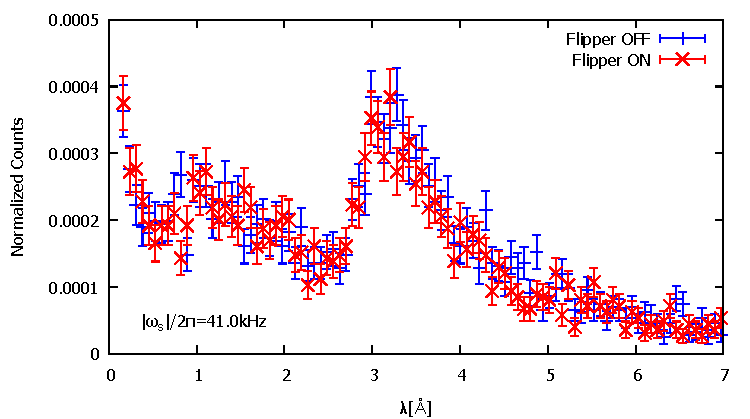
\includegraphics[height=4.3cm]{resonance/analysis/Flipper1_NormalizedCounts_410kHz.pdf}
%\vspace{4.3cm}
%\end{minipage}
\caption{上流フリッパー共鳴実験における規格化粒子数の波長分布}\label{Resonance_fig_Flipper1_NormalizedCounts}
\end{figure}

さらに、図\ref{Resonance_fig_Flipper1_CountsRate}にフリッパーONのときの規格化粒子数をフリッパーOFFのときの規格化粒子数で割ったもの、すなわち上流フリッパーでスピン反転しなかった割合の波長分布を表す。図\ref{Resonance_fig_Flipper1_CountsRate}を見ると、波長$\lambda=$3.0{\AA}から4.5{\AA}あたりで大きく凹んでいることがわかる。
\begin{figure}[h]
%\begin{minipage}{0.49\hsize}
%\centering
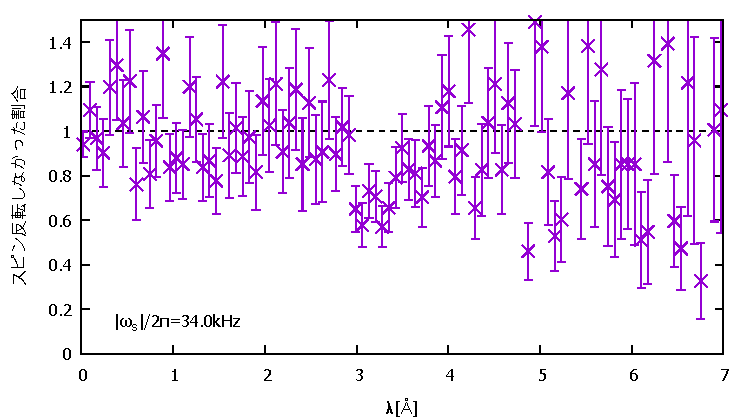
\includegraphics[height=4.3cm]{resonance/analysis/Flipper1_CountsRate_340kHz.pdf}
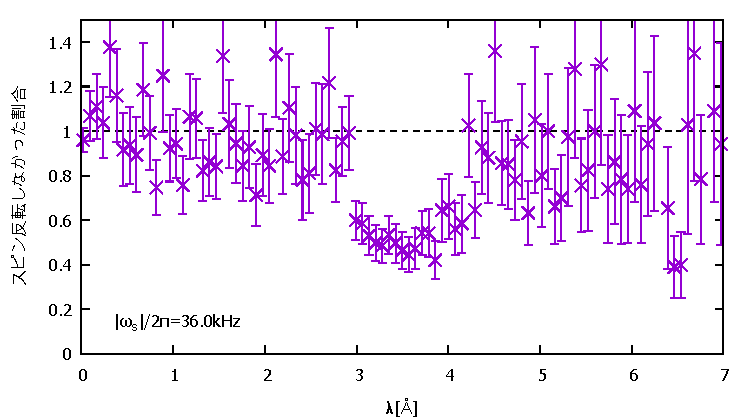
\includegraphics[height=4.3cm]{resonance/analysis/Flipper1_CountsRate_360kHz.pdf}\\
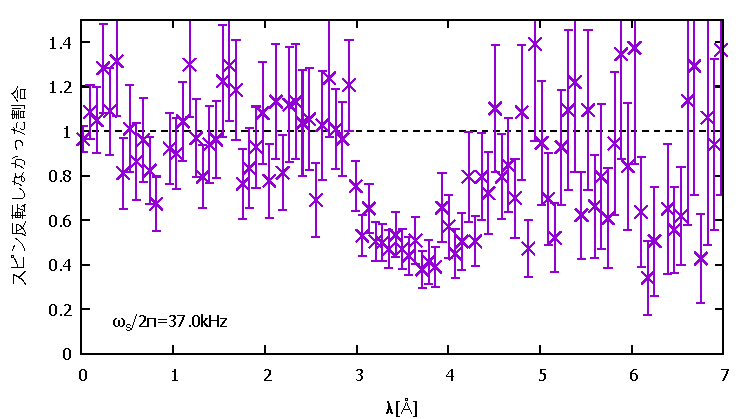
\includegraphics[height=4.3cm]{resonance/analysis/Flipper1_CountsRate_370kHz.pdf}
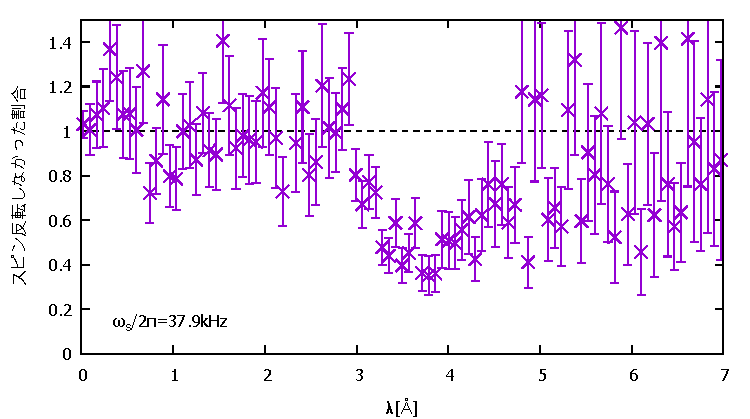
\includegraphics[height=4.3cm]{resonance/analysis/Flipper1_CountsRate_379kHz.pdf}\\
%\end{minipage}
%\begin{minipage}{0.49\hsize}
%\centering
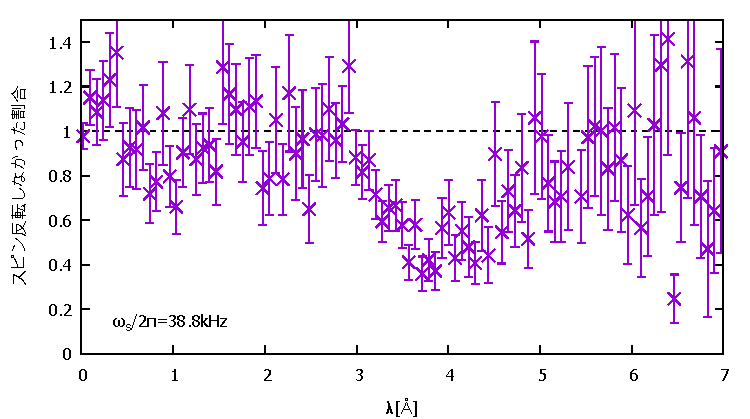
\includegraphics[height=4.3cm]{resonance/analysis/Flipper1_CountsRate_388kHz.pdf}
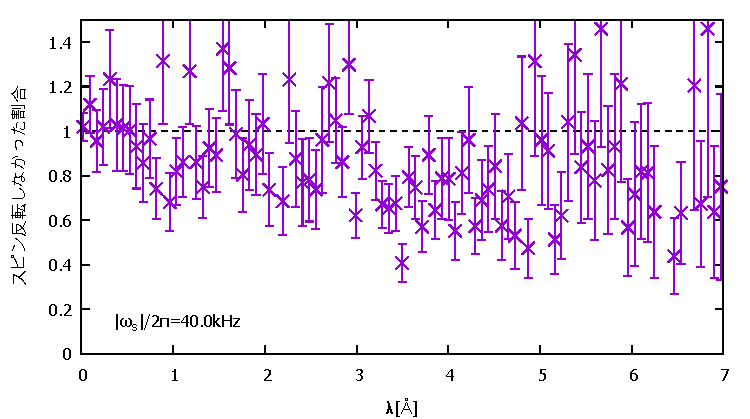
\includegraphics[height=4.3cm]{resonance/analysis/Flipper1_CountsRate_400kHz.pdf}\\
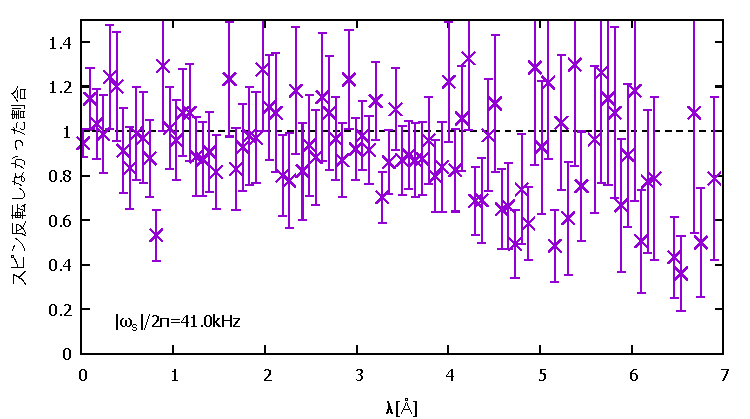
\includegraphics[height=4.3cm]{resonance/analysis/Flipper1_CountsRate_410kHz.pdf}
%\vspace{4.3cm}
%\end{minipage}
\caption{上流フリッパーにおいてスピン反転しなかった割合}\label{Resonance_fig_Flipper1_CountsRate}
\end{figure}

そこで、図\ref{Resonance_fig_Flipper1_NormalizedCounts}の波長領域$\lambda=$3.0{\AA}から4.5{\AA}における規格化粒子数の和を$|\omega_s|/2\pi$を横軸に取って図示すると図\ref{Resonance_fig_Flipper1_Freq}のようになる。2次関数でフィッティングした結果、最もカウントが少なくなる、すなわち共鳴条件(\ref{Resonance_resonance})を満たす$\omega_s$として$|\omega_s|/2\pi=37.17\pm0.03$kHzと決まった。
\begin{comment}
\begin{table}[h]
\centering
\begin{tabular}{c|lllllll}
$|\omega_s|/2\pi$&34.0&36.0&37.0&37.9&38.8&40.0&41.0\\
$3.0{\AA}-4.5{\AA}での規格化粒子数($\times 10^{-4}$)&$17.8\pm0.8$&18.4\pm
\end{comment}
\begin{figure}[h]
\centering
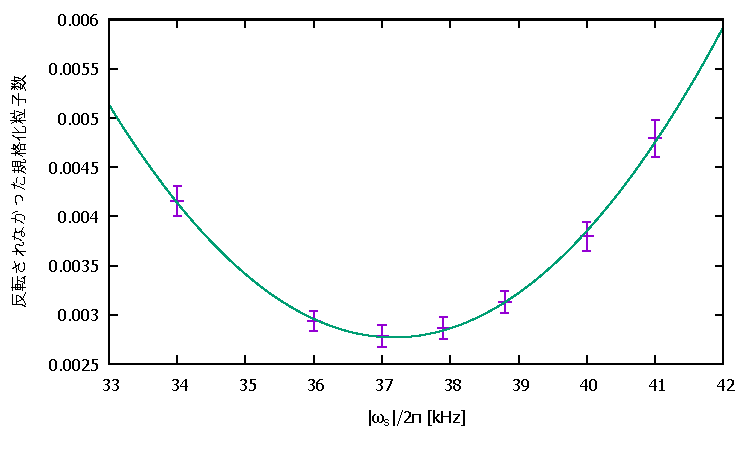
\includegraphics[width=12cm]{resonance/analysis/Flipper1_Freq_30-45r.pdf}
\caption{$|\omega_s|/2\pi$に対する波長$\lambda=$3.0{\AA}から4.5{\AA}における規格化粒子数}\label{Resonance_fig_Flipper1_Freq}
\end{figure}

次に、決まった$\omega_s$と最も近い$|\omega_s|/2\pi=37.0$kHzのときのスピン反転しなかった割合の波長分布(図\ref{Resonance_fig_Flipper1_CountsRate_370fit})から、最も反転しない割合が低い、すなわち最も反転する波長を推定すると、2次関数フィットの結果、$\lambda=3.66\pm0.05${\AA}と求まった。これを速度に直すと$v=1080\pm15$m/sとなり、この速度が$\pi$フリップ条件(\ref{Resonance_piflip})を満たすことから$\omega_{r1}/2\pi=9.0\pm0.1$kHzと計算される。
\begin{figure}[h]
\centering
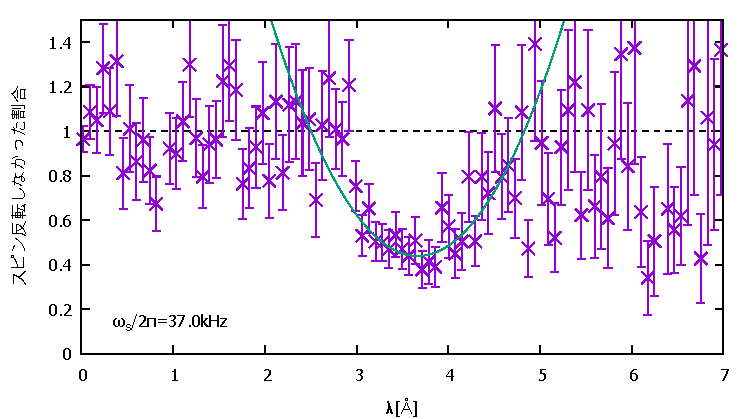
\includegraphics[width=12cm]{resonance/analysis/Flipper1_CountsRate_370kHz_fit.pdf}
\caption{$|\omega_s|/2\pi$=37.0kHzのときのスピン反転しなかった割合の波長分布}\label{Resonance_fig_Flipper1_CountsRate_370fit}
\end{figure}

\paragraph{下流フリッパーに関する分析}
上流フリッパー同様に下流フリッパーの測定データについても互いに比較するために、測定時間のLiMカウントで規格化を行う。その結果を図\ref{Resonance_fig_Flipper2_NormalizedCounts}に表す。
\begin{figure}[h]
%\begin{minipage}{0.49\hsize}
%\centering
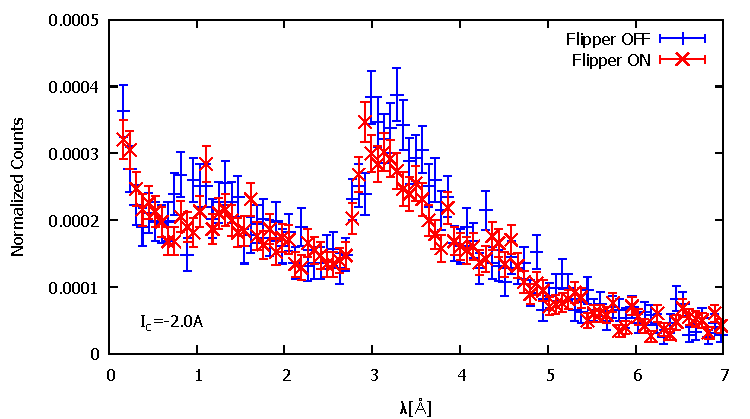
\includegraphics[height=4.3cm]{resonance/analysis/Flipper2_NormalizedCounts_-20A.pdf}
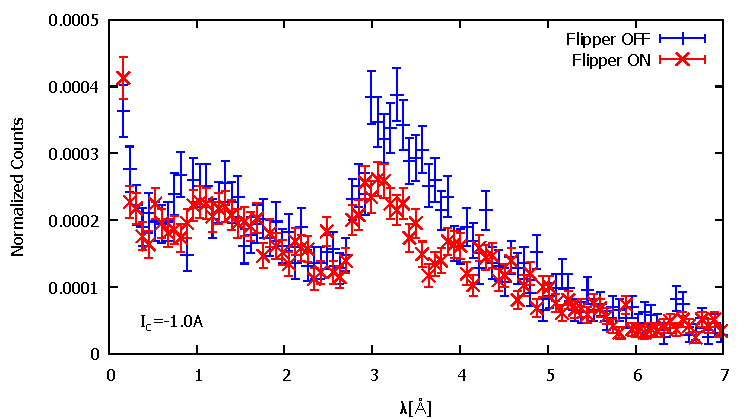
\includegraphics[height=4.3cm]{resonance/analysis/Flipper2_NormalizedCounts_-10A.pdf}\\
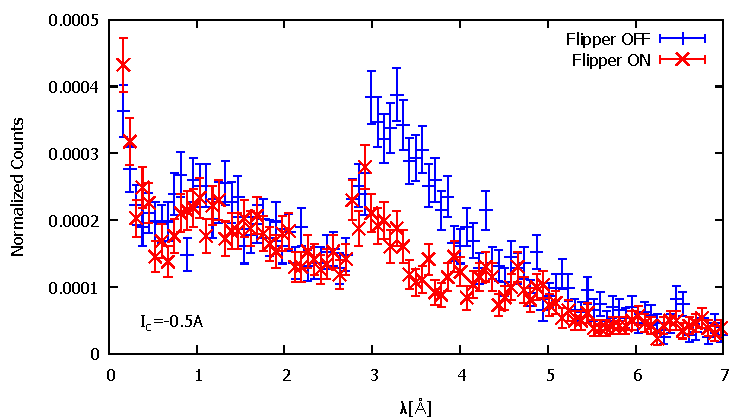
\includegraphics[height=4.3cm]{resonance/analysis/Flipper2_NormalizedCounts_-5A.pdf}
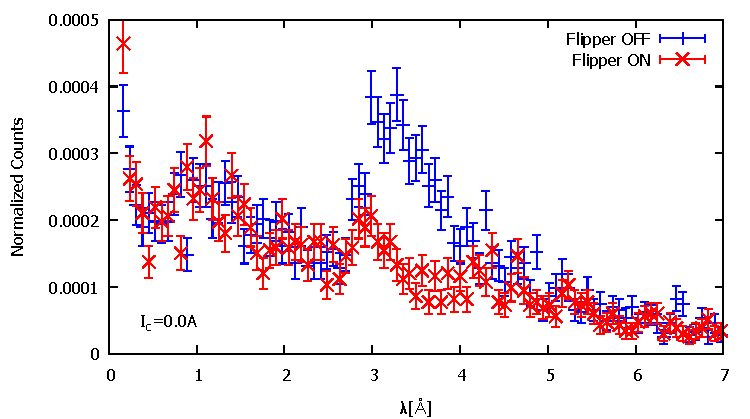
\includegraphics[height=4.3cm]{resonance/analysis/Flipper2_NormalizedCounts_0A.pdf}\\
%\end{minipage}
%\begin{minipage}{0.49\hsize}
%\centering
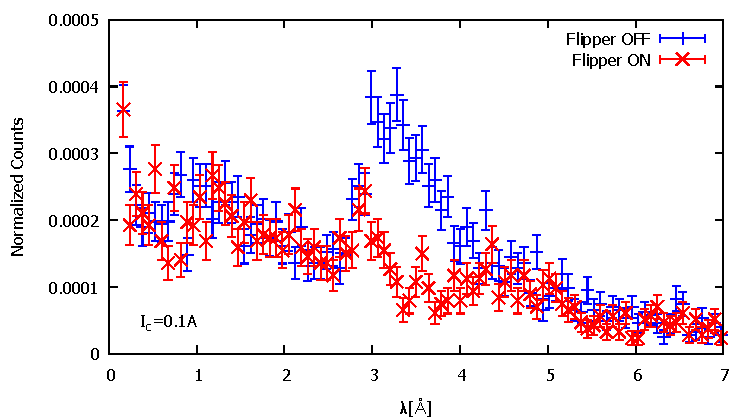
\includegraphics[height=4.3cm]{resonance/analysis/Flipper2_NormalizedCounts_1A.pdf}
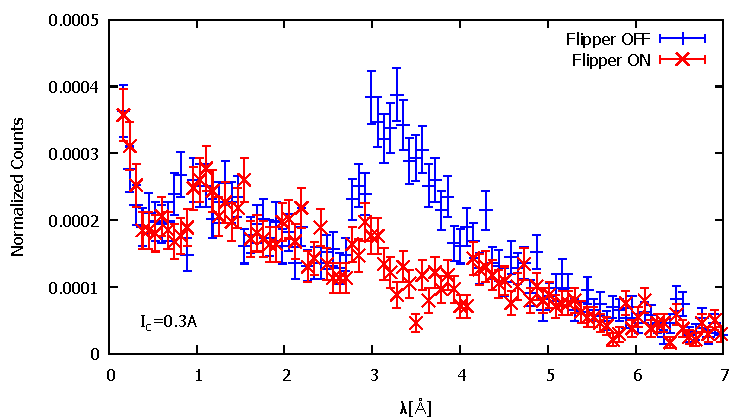
\includegraphics[height=4.3cm]{resonance/analysis/Flipper2_NormalizedCounts_3A.pdf}\\
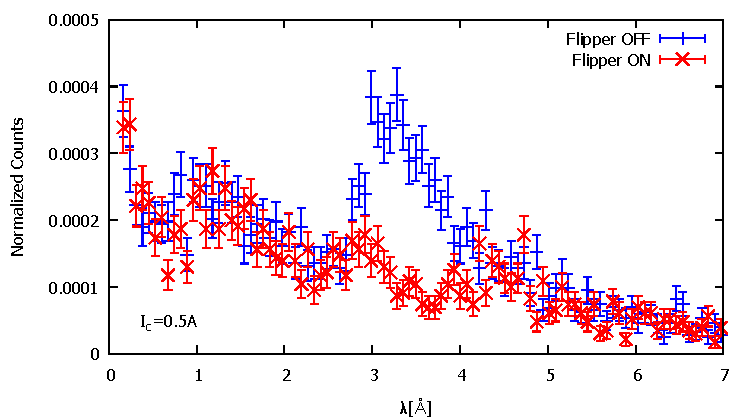
\includegraphics[height=4.3cm]{resonance/analysis/Flipper2_NormalizedCounts_5A.pdf}
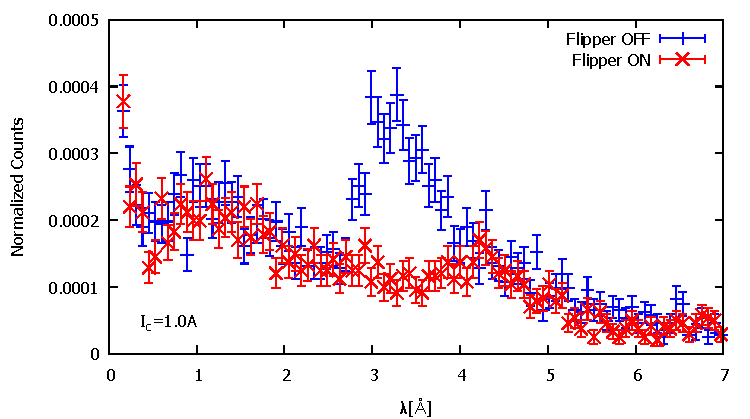
\includegraphics[height=4.3cm]{resonance/analysis/Flipper2_NormalizedCounts_10A.pdf}\\
%\vspace{4.3cm}
%\end{minipage}
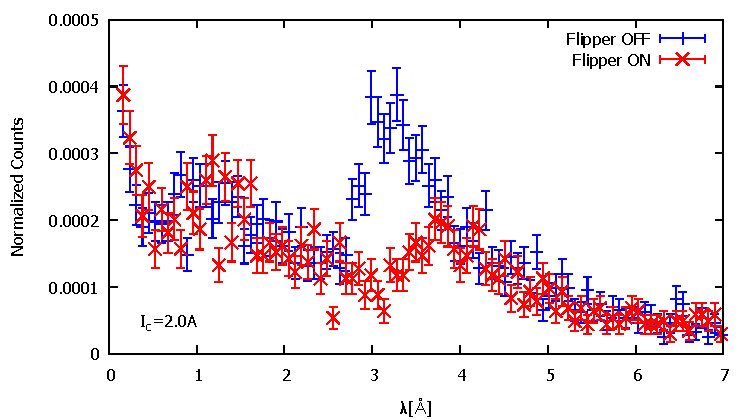
\includegraphics[height=4.3cm]{resonance/analysis/Flipper2_NormalizedCounts_20A.pdf}
\caption{下流フリッパー共鳴実験における規格化粒子数の波長分布}\label{Resonance_fig_Flipper2_NormalizedCounts}
\end{figure}

さらに、図\ref{Resonance_fig_Flipper2_CountsRate}にフリッパーONのときの規格化粒子数をフリッパーOFFのときの規格化粒子数で割ったもの、すなわち上流フリッパーでスピン反転しなかった割合の波長分布を表す。図\ref{Resonance_fig_Flipper2_CountsRate}を見ると、波長$\lambda=$3.0{\AA}から4.0{\AA}あたりで大きく凹んでいることがわかる。
\begin{figure}[h]
%\begin{minipage}{0.49\hsize}
%\centering
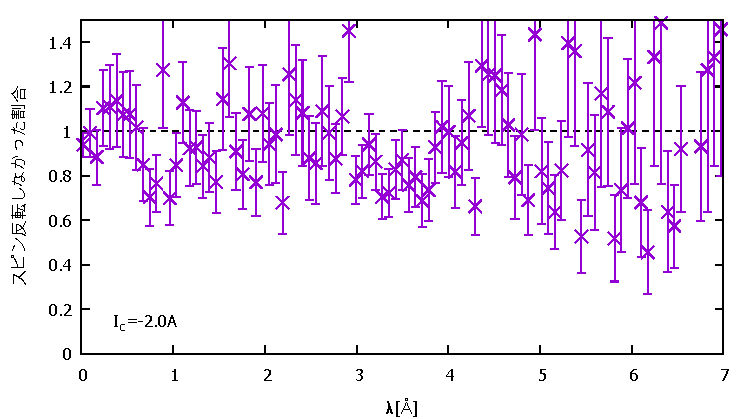
\includegraphics[height=4.3cm]{resonance/analysis/Flipper2_CountsRate_-20A.pdf}
\includegraphics[height=4.3cm]{resonance/analysis/Flipper2_CountsRate_-10A.pdf}\\
\includegraphics[height=4.3cm]{resonance/analysis/Flipper2_CountsRate_-5A.pdf}
\includegraphics[height=4.3cm]{resonance/analysis/Flipper2_CountsRate_0A.pdf}\\
%\end{minipage}
%\begin{minipage}{0.49\hsize}
%\centering
\includegraphics[height=4.3cm]{resonance/analysis/Flipper2_CountsRate_1A.pdf}
\includegraphics[height=4.3cm]{resonance/analysis/Flipper2_CountsRate_3A.pdf}\\
\includegraphics[height=4.3cm]{resonance/analysis/Flipper2_CountsRate_5A.pdf}
\includegraphics[height=4.3cm]{resonance/analysis/Flipper2_CountsRate_10A.pdf}\\
%\vspace{4.3cm}
%\end{minipage}
\includegraphics[height=4.3cm]{resonance/analysis/Flipper2_CountsRate_20A.pdf}
\caption{下流フリッパーにおいてスピン反転しなかった割合}\label{Resonance_fig_Flipper2_CountsRate}
\end{figure}

そこで、図\ref{Resonance_fig_Flipper2_NormalizedCounts}の波長領域$\lambda=$2.7{\AA}から4.2{\AA}における規格化粒子数を数え、$I_c$を横軸として図示すると図\ref{Resonance_fig_Flipper2_Cur}のようになる。2次関数でフィッティングした結果、最もカウントが少なくなる、すなわち共鳴条件(\ref{Resonance_resonance})を満たす$I_c$として$I_c=0.7\pm0.1$Aと決まった。
\begin{figure}[h]
\centering
\includegraphics[width=12cm]{resonance/analysis/Flipper2_Cur_30-40.pdf}
\caption{$I_c$に対する波長$\lambda=$3.0{\AA}から4.0{\AA}における規格化粒子数}\label{Resonance_fig_Flipper2_Cur}
\end{figure}

次に、決まった$I_c$の中心値と最も近い$I_c=0.7$Aのときのスピン反転しなかった割合の波長分布(図\ref{Resonance_fig_Flipper2_CountsRate_7fit})から、最も反転しない割合が低い、すなわち最も反転する波長を推定すると、2次関数フィットの結果、$\lambda=3.40\pm0.03${\AA}と求まった。これを速度に直すと$v=1163\pm10$m/sとなり、この速度が$\pi$フリップ条件(\ref{Resonance_piflip})を満たすことから$\omega_{r2}/2\pi=9.6\pm0.1$kHzと計算される。
\begin{figure}[h]
\centering
\includegraphics[width=12cm]{resonance/analysis/Flipper2_CountsRate_7A_fit.pdf}
\caption{$I_c$=0.7Aのときのスピン反転しなかった割合の波長分布}\label{Resonance_fig_Flipper2_CountsRate_7fit}
\end{figure}

\clearpage
\paragraph{分析まとめ}
以上の分析から各パラメータは次のように決まった。
\begin{table}[h]
\centering
\begin{tabular}{|c|c|} \hline
$|\omega_s|/2\pi$&$37.17\pm0.03$kHz\\ \hline
$I_c$&$0.7\pm0.1$A \\ \hline
$\omega_{r1}/2\pi$&$9.0\pm0.1$kHz \\ \hline
$\omega_{r2}/2\pi$&$9.6\pm0.1$kHz \\ \hline
\end{tabular}
\end{table}

しかし、実験中の粗い解析では$|\omega_s|/2\pi=37.5\pm0.1$kHz,$I_c=0.185\pm0.11$Aと求まったため、実際には以後、
\begin{table}[h]
\centering
\begin{tabular}{|c|c|} \hline
$|\omega_s|/2\pi$&37.5kHz\\ \hline
$I_c$&0.185A \\ \hline
\end{tabular}
\end{table}

\noindent として実験を進めた。このことによる共鳴条件からのずれは最大で$\epsilon/|\omega_z|=$0.1程度であり、十分小さいといえる(図\ref{Resonance_fig_visivility},\ref{Resonance_fig_interference}参照)。
